\documentclass[../main.tex]{subfiles}
%!TEX root = ./analysisConnector.tex
\graphicspath {{../}}

\begin{document}
\subsection{Connection To Keel} \label{connector}
\begin{figure}[H]
	\centering
	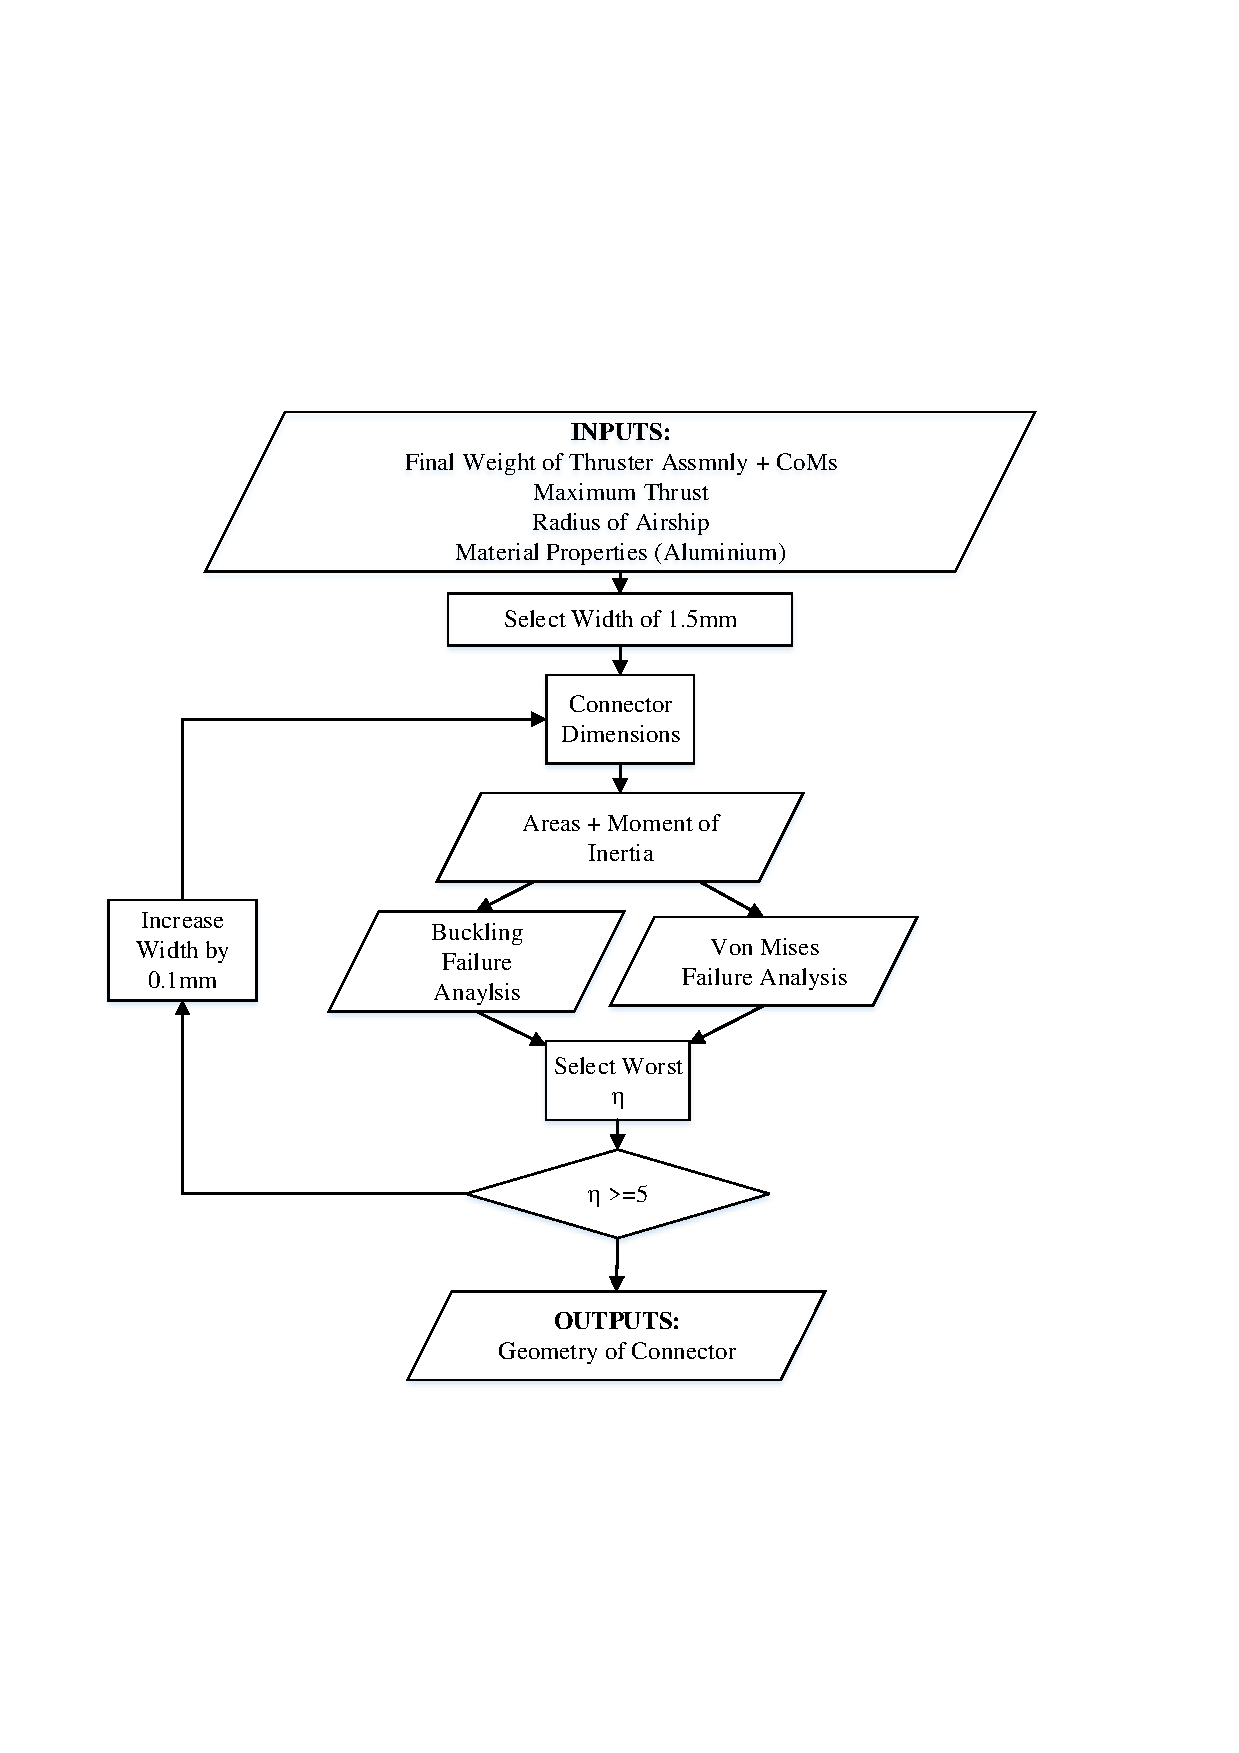
\includegraphics[width=.9\linewidth]{img/paramaterization/connector.pdf}
	\caption{Parametrization Outline for the Thruster Arm Connector}
	\label{fig:connectorParametrization}
\end{figure}

This section analyzes the thruster arms connection to the keel. It uses a rectangular piece that attaches into the bottom of the arm and the piece used for connecting the sections of keel together. The analysis outputs the geometry of the connector piece such that it meets the safety factor of 5 assigned to the component. The inputs required in order to preform the analysis include, the final weight of thruster assembly and its center of mass data, the radius of the thruster arms and the material properties aluminum 6061 \cite{AlProperties}. 

The first analysis relates to the System Modelling Loading Scenario section \ref{loadingScenarios} Maximum Downward Force Figure \ref{fig:scenario1}. In this scenario the connector holds the weight and thrusting forces in the x direction. The assumption is that the two failures can occur from buckling and bending of the piece. A free body diagram of the top of the connector can be seen in Figure ???. The analysis begins by solving the reaction forces and moments acting on the connector piece using the weights ??? function ref?? and forceSolver???. 

\begin{equation}
\label{eqn:connectorztress}
\sigma_{z}=  \underbrace{\frac{M_{x}c_y}{I_x}}_\text{Bending moment stress about x} + \underbrace{\frac{M_{y}c_x}{I_y}}_\text{Bending moment stress about z} + \underbrace{\frac{F_z}{A}}_\text{Axial stress} 
\end{equation}
Because of the loading scenario both $F_y$ and $M_z$ are zero and there for do not contribute to the total stress. In addition to the planar stress in z there is also torsional shear in the xy plane. This is describes by equation \ref{eqn:armtorsionShear} from {(Shigley's Machine Design \cite[102]{shigley})}.
\begin{equation} \label{eqn:armtorsionShear}
\tau_{xy} = \dfrac{M_{z}}{wt^2}(3+\frac{1.8t}{w})
\end{equation}
The equation accounts for the maximum shear stress in a rectangular cross section which occurs in the center of the wider side which in this case is the width. \\ 

Next the analysis takes both the planar and shear stresses and convertes them to principle stresses (as shown in Appendix \ref{appendix:cauchy}). These principle stresses are then used to determine the safety factor by Von Mises Theory \cite[221]{shigley}.

\begin{equation}
\eta = \dfrac{S_{ut}}{\sigma _a} \Rightarrow 5 \geq \dfrac{S_{ut}}{\sigma _a}
\end{equation}

A safety factor of five was chosen because there is a relatively high failure likelihood and a failure of this component would result in catastrophic failure of the airship.\\

For the buckling failure, this could occur at the top part of the connector. Using the reaction forces found in Force Calculation section the cross section can be drawn, seen in Figure ?? The buckling is calculated using Euler's critical load cite??. 

\begin{equation} \label{eqn:EulersCriticalForce}
P_{cr} = \frac{C\pi^2EI_z}{l^2}
\end{equation}
Where $C$ is an end constant taken as $1.2$ for this case, $E$ is the modulus of elasticity, $l$ is the height shown in Figure ??, and $I_z$ is calculated using:
\begin{equation}
I_z = \frac{b^3l}{12}
\end{equation}
Plugging these values into Equation \ref{eqn:EulersCriticalForce}:
\begin{equation}
P_{cr} = \frac{(1.2)\pi^2Eb^3}{12l}
\end{equation}
The safety factor is calculated using the force applied and the critical force (Equation \ref{eqn:EulersCriticalForce}):
\begin{equation}
\eta = \frac{P_{cr}}{F_{Rz}}
\end{equation}
\paragraph*{Sample Calculations}
$M_y$ and $F_{Rz}$ values taken from the MATLAB Force Solver.
$$\sigma_{z}={\frac{M_{x}c_y}{I_x}}+{\frac{M_{y}c_x}{I_y}}+{\frac{F_z}{A}}$$
$$\sigma_{z}=0+\frac{(17.2196N\cdot{}m)(0.0200m)}{8.000\cdot{}10^{-9}mm^4}+0 = 43.049MPa$$
$$\eta = \dfrac{S_{ut}}{\sigma _a} = \dfrac{310MPa}{43.049MPa}=7.2$$
$$P_{cr} = \frac{(1.2)\pi^2Eb^3}{12l}=\frac{(1.2)\pi^2(68.9\cdot{}10^9Pa)(0.0015m)^3}{12(0.0330m)}=6954.71N$$
$$\eta = \frac{P_{cr}}{F_{Rz}} = \frac{6954.71N}{29.9623N} = 232$$

\end{document}